\documentclass{standalone}
\usepackage{tikz}
\usetikzlibrary{patterns, positioning}
\usepackage[sfdefault]{ClearSans} %% option 'sfdefault' activates Clear Sans as the default text font
\usepackage[T1]{fontenc}

\begin{document}
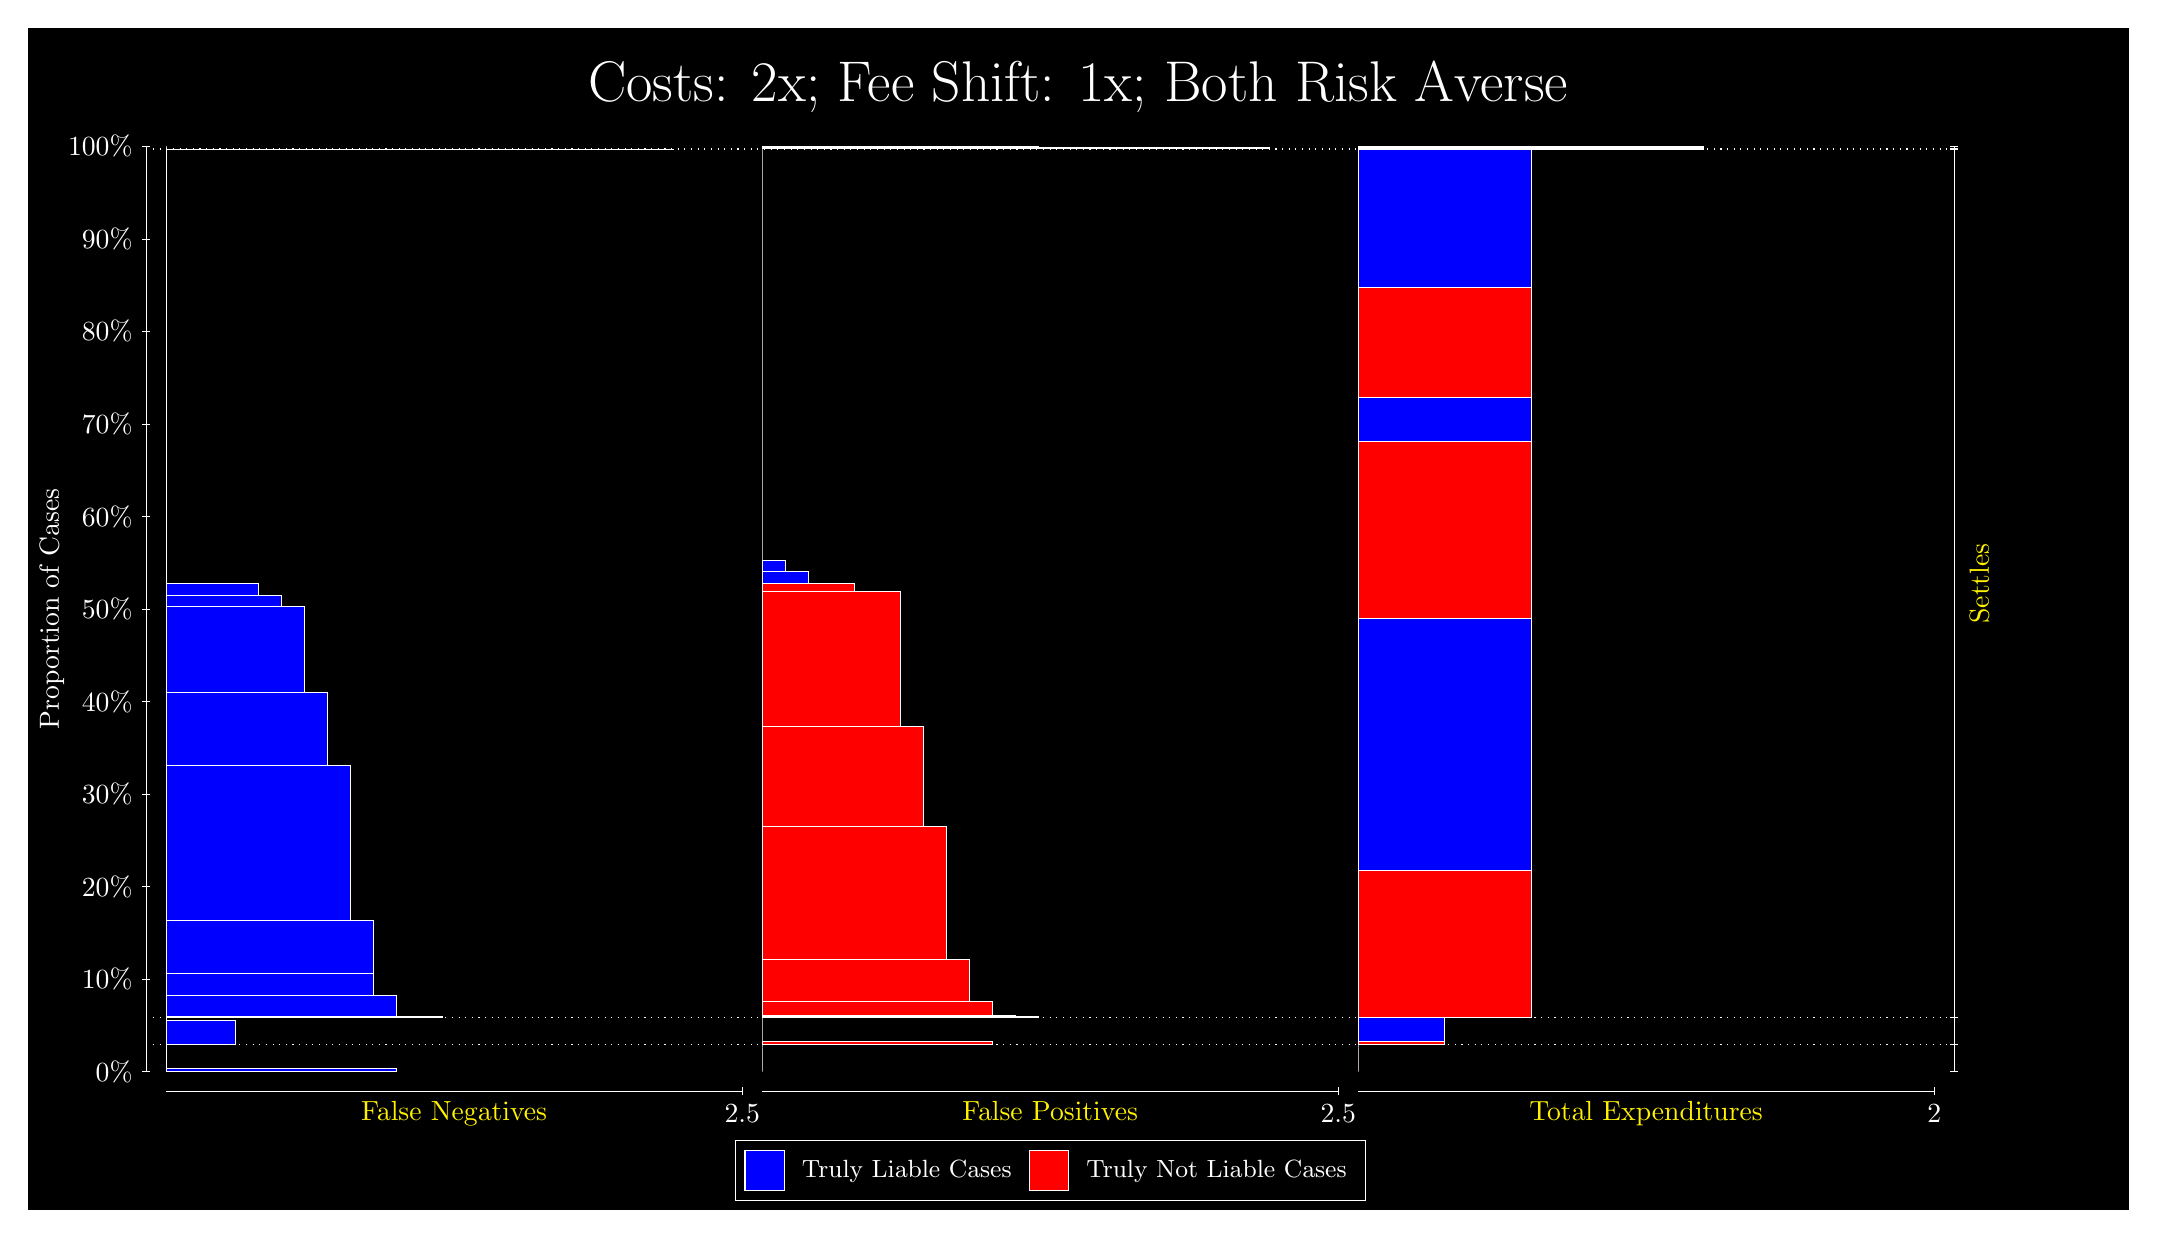
\begin{tikzpicture}
\draw[fill=black] (0,0) rectangle (26.667,15);
\draw[text=white] (0,13.5) rectangle (26.667,15) node[midway] {\huge Costs: 2x; Fee Shift: 1x; Both Risk Averse};
\draw[white, very thin] (1.5,1.75) -- (1.5,13.5);
\node[rotate=90, text=white, anchor=center] at (0.3, 7.625) {Proportion of Cases};
\draw[white, very thin] (1.45,1.75) -- (1.55,1.75);
\node[text=white, anchor=east] at (1.45, 1.75) {0\%};
\draw[white, very thin] (1.45,2.925) -- (1.55,2.925);
\node[text=white, anchor=east] at (1.45, 2.925) {10\%};
\draw[white, very thin] (1.45,4.1) -- (1.55,4.1);
\node[text=white, anchor=east] at (1.45, 4.1) {20\%};
\draw[white, very thin] (1.45,5.275) -- (1.55,5.275);
\node[text=white, anchor=east] at (1.45, 5.275) {30\%};
\draw[white, very thin] (1.45,6.45) -- (1.55,6.45);
\node[text=white, anchor=east] at (1.45, 6.45) {40\%};
\draw[white, very thin] (1.45,7.625) -- (1.55,7.625);
\node[text=white, anchor=east] at (1.45, 7.625) {50\%};
\draw[white, very thin] (1.45,8.8) -- (1.55,8.8);
\node[text=white, anchor=east] at (1.45, 8.8) {60\%};
\draw[white, very thin] (1.45,9.975) -- (1.55,9.975);
\node[text=white, anchor=east] at (1.45, 9.975) {70\%};
\draw[white, very thin] (1.45,11.15) -- (1.55,11.15);
\node[text=white, anchor=east] at (1.45, 11.15) {80\%};
\draw[white, very thin] (1.45,12.325) -- (1.55,12.325);
\node[text=white, anchor=east] at (1.45, 12.325) {90\%};
\draw[white, very thin] (1.45,13.5) -- (1.55,13.5);
\node[text=white, anchor=east] at (1.45, 13.5) {100\%};

\draw[white, very thin] (24.457,1.75) -- (24.457,13.5);
\draw[white, very thin] (24.407,1.75) -- (24.507,1.75);
\node[anchor=west] at (24.407, 1.75) {};
\draw[white, very thin] (24.407,2.0934) -- (24.507,2.0934);
\node[anchor=west] at (24.407, 2.0934) {};
\draw[white, very thin] (24.407,2.4368) -- (24.507,2.4368);
\node[anchor=west] at (24.407, 2.4368) {};
\draw[white, very thin] (24.407,13.459) -- (24.507,13.459);
\node[anchor=west] at (24.407, 13.459) {};
\draw[white, very thin] (24.407,13.477) -- (24.507,13.477);
\node[anchor=west] at (24.407, 13.477) {};
\draw[white, very thin] (24.407,13.5) -- (24.507,13.5);
\node[anchor=west] at (24.407, 13.5) {};

\draw[white, very thin, fill=blue] (1.75,1.75) rectangle (4.6775,1.7861);
\draw[white, very thin, fill=red] (1.75,1.7861) rectangle (1.75,2.0934);
\draw[white, very thin, fill=blue] (1.75,2.0934) rectangle (2.6283,2.4007);
\draw[white, very thin, fill=red] (1.75,2.4007) rectangle (1.75,2.4368);
\draw[white, very thin, fill=blue] (1.75,2.4368) rectangle (5.2631,2.4507);
\draw[white, very thin, fill=blue] (1.75,2.4507) rectangle (4.6775,2.7152);
\draw[white, very thin, fill=blue] (1.75,2.7152) rectangle (4.3848,2.9984);
\draw[white, very thin, fill=blue] (1.75,2.9984) rectangle (4.3848,3.6747);
\draw[white, very thin, fill=blue] (1.75,3.6747) rectangle (4.092,5.6376);
\draw[white, very thin, fill=blue] (1.75,5.6376) rectangle (3.7993,6.5657);
\draw[white, very thin, fill=blue] (1.75,6.5657) rectangle (3.5065,7.6595);
\draw[white, very thin, fill=blue] (1.75,7.6595) rectangle (3.2138,7.7978);
\draw[white, very thin, fill=blue] (1.75,7.7978) rectangle (2.921,7.9453);
\draw[white, very thin, fill=red] (1.75,7.9453) rectangle (1.75,13.459);
\draw[white, very thin, fill=blue] (1.75,13.459) rectangle (8.1906,13.466);
\draw[white, very thin, fill=red] (1.75,13.466) rectangle (1.75,13.477);
\draw[white, very thin, fill=red] (1.75,13.477) rectangle (1.75,13.484);
\draw[white, very thin, fill=blue] (1.75,13.484) rectangle (1.75,13.5);
\draw[white, very thin, fill=red] (9.3189,1.75) rectangle (9.3189,2.0572);
\draw[white, very thin, fill=blue] (9.3189,2.0572) rectangle (9.3189,2.0934);
\draw[white, very thin, fill=red] (9.3189,2.0934) rectangle (12.246,2.1295);
\draw[white, very thin, fill=blue] (9.3189,2.1295) rectangle (9.3189,2.4368);
\draw[white, very thin, fill=red] (9.3189,2.4368) rectangle (12.832,2.455);
\draw[white, very thin, fill=red] (9.3189,2.455) rectangle (12.539,2.4687);
\draw[white, very thin, fill=red] (9.3189,2.4687) rectangle (12.246,2.6464);
\draw[white, very thin, fill=red] (9.3189,2.6464) rectangle (11.954,3.1817);
\draw[white, very thin, fill=red] (9.3189,3.1817) rectangle (11.661,4.8648);
\draw[white, very thin, fill=red] (9.3189,4.8648) rectangle (11.368,6.135);
\draw[white, very thin, fill=red] (9.3189,6.135) rectangle (11.075,7.8466);
\draw[white, very thin, fill=red] (9.3189,7.8466) rectangle (10.49,7.9507);
\draw[white, very thin, fill=blue] (9.3189,7.9507) rectangle (9.9044,8.0981);
\draw[white, very thin, fill=blue] (9.3189,8.0981) rectangle (9.6116,8.2365);
\draw[white, very thin, fill=blue] (9.3189,8.2365) rectangle (9.3189,13.459);
\draw[white, very thin, fill=red] (9.3189,13.459) rectangle (9.3189,13.47);
\draw[white, very thin, fill=blue] (9.3189,13.47) rectangle (9.3189,13.477);
\draw[white, very thin, fill=red] (9.3189,13.477) rectangle (15.759,13.484);
\draw[white, very thin, fill=blue] (9.3189,13.484) rectangle (12.832,13.5);
\draw[white, very thin, fill=red] (16.888,1.75) rectangle (16.888,2.0572);
\draw[white, very thin, fill=blue] (16.888,2.0572) rectangle (16.888,2.0934);
\draw[white, very thin, fill=red] (16.888,2.0934) rectangle (17.986,2.1295);
\draw[white, very thin, fill=blue] (16.888,2.1295) rectangle (17.986,2.4368);
\draw[white, very thin, fill=red] (16.888,2.4368) rectangle (19.083,4.3114);
\draw[white, very thin, fill=blue] (16.888,4.3114) rectangle (19.083,7.5064);
\draw[white, very thin, fill=red] (16.888,7.5064) rectangle (19.083,9.7556);
\draw[white, very thin, fill=blue] (16.888,9.7556) rectangle (19.083,10.317);
\draw[white, very thin, fill=red] (16.888,10.317) rectangle (19.083,11.707);
\draw[white, very thin, fill=blue] (16.888,11.707) rectangle (19.083,13.459);
\draw[white, very thin, fill=red] (16.888,13.459) rectangle (21.279,13.47);
\draw[white, very thin, fill=blue] (16.888,13.47) rectangle (21.279,13.477);
\draw[white, very thin, fill=red] (16.888,13.477) rectangle (21.279,13.484);
\draw[white, very thin, fill=blue] (16.888,13.484) rectangle (21.279,13.5);
\draw[white, dotted] (1.5,2.0934) -- (24.457,2.0934);
\draw[white, dotted] (1.5,2.4368) -- (24.457,2.4368);
\draw[white, dotted] (1.5,13.459) -- (24.457,13.459);
\draw[white, dotted] (1.5,13.477) -- (24.457,13.477);
\draw[white, very thin] (1.75,1.5) -- (9.0689,1.5);
\node[text=yellow, anchor=north] at (5.4094, 1.5) {False Negatives};
\draw[white, very thin] (9.0689,1.45) -- (9.0689,1.55);
\node[text=white, anchor=north] at (9.0689, 1.45) {2.5};

\draw[white, very thin] (9.3189,1.5) -- (16.638,1.5);
\node[text=yellow, anchor=north] at (12.978, 1.5) {False Positives};
\draw[white, very thin] (16.638,1.45) -- (16.638,1.55);
\node[text=white, anchor=north] at (16.638, 1.45) {2.5};

\draw[white, very thin] (16.888,1.5) -- (24.207,1.5);
\node[text=yellow, anchor=north] at (20.547, 1.5) {Total Expenditures};
\draw[white, very thin] (24.207,1.45) -- (24.207,1.55);
\node[text=white, anchor=north] at (24.207, 1.45) {2};



\node[text=yellow, centered, rotate=90] at (24.777, 7.948) {Settles};



\draw (12.978300999999998,1.5) node[draw=none] (baseCoordinate) {};
\begin{scope}[align=center]
        \matrix[scale=0.5, draw=white, below=0.5cm of baseCoordinate, nodes={draw}, column sep=0.1cm]{
            \node[rectangle, draw, minimum width=0.5cm, minimum height=0.5cm, fill=blue] {}; &
            \node[draw=none, font=\small, text=white] (B) {Truly Liable Cases}; &
            \node[rectangle, draw, minimum width=0.5cm, minimum height=0.5cm, fill=red] {}; &
            \node[draw=none, font=\small, text=white] (B) {Truly Not Liable Cases}; \\
            };
\end{scope}

\end{tikzpicture}
\end{document}